% arara: xelatex
% arara: xelatex
% arara: xelatex

% options:
% thesis=B bachelor's thesis
% thesis=M master's thesis
% czech thesis in Czech language
% english thesis in English language
% hidelinks remove colour boxes around hyperlinks

\documentclass[thesis=M,english]{FITthesis}[2012/10/20]

\usepackage[utf8]{inputenc}

\usepackage{graphicx} %graphics files inclusion
% \usepackage{subfig} %subfigures
% \usepackage{amsmath} %advanced maths
% \usepackage{amssymb} %additional math symbols

\usepackage{dirtree} %directory tree visualisation

% ADDED BY ME
\usepackage{blindtext} % lorem ipsum
\usepackage{todonotes} 

\newcommand{\todotext}[1]{\textcolor{red}{\textbf{[[#1]]}}}
\newcommand{\redtext}[1]{\textcolor{red}{[[#1]]}}
\definecolor{mygray}{gray}{0.6}
\newcommand{\blind}[1][1]{\textcolor{mygray}{\Blindtext[#1][1]}}

\setlength{\fboxsep}{0.005pt}
\newcommand{\tmpframe}[1]{\fbox{#1}}
%\renewcommand{\tmpframe}[1]{#1}

\let\myCite\cite
\renewcommand\cite{\unskip~\myCite}
\let\myRef\ref
\renewcommand\ref{\unskip~\myRef}

% \usepackage{spverbatim} % verb and verbatim with line breaks - doesn't break what I need

\newcommand\hatx{\^{}}



% list of acronyms
%\usepackage[acronym,nonumberlist,toc,numberedsection=autolabel,nomain]{glossaries}
\iflanguage{czech}{\renewcommand*{\acronymname}{Seznam pou{\v z}it{\' y}ch zkratek}}{}
%\makeglossaries

\newcommand{\tg}{\mathop{\mathrm{tg}}} %cesky tangens
\newcommand{\cotg}{\mathop{\mathrm{cotg}}} %cesky cotangens

% % % % % % % % % % % % % % % % % % % % % % % % % % % % % % % % % % % 
% % % % % % % % % % % % % % % % % % % % % % % % % % % % % % % % % % % 
\department{Department of theoretical computer science}
\title{Contextual Shell History}
\authorGN{Šimon} %author's given name/names
\authorFN{Let} %author's surname
\authorWithDegrees{Bc. Šimon Let} %author's name with academic degrees
\author{Šimon Let} %author's name without academic degrees
\supervisor{Ing. Lukáš Bařinka}
% my BP thesis: I~would like to thank my supervisor Ing. V{\' i}t List{\' i}k, without his assistance and guidance this thesis would have not be accomplished.
% \par Then I~would like to thank Ing. Michal Bukovsk{\' y} along with his whole Email.cz team in Seznam.cz for letting me work with them and use their data.
% \par My thanks also goes to RNDr. Jana Strakov{\' a} at. el for developing Nametag, Named entity recognition solution, I~used in this thesis, and answering my questions.
% \par Finally I~want to thank my family and friends for their support trough my whole studies.
\acknowledgements{\todotext{TODO: I would like to thank my supervisor Ing. Lukáš Bařinka for his guidance, my colleagues and friends for their feedback, hundreds of people who downloaded this project for their trust, and my family for support during writing this thesis. Installfest for accepting my talk about this project. Github users who submitted issues and pull requests to the project.}}
\abstractCS{\todotext{TODO: CZ abstrakt}  \blind[2]}
\abstractEN{\todotext{TODO: abstract} This thesis is an enhancement for standard shell history. It records shell history with context. It uses the recorded context to make it easier to find relevant history records and to make it possible to search search history using context explicitly.

\blind[2]
}
\placeForDeclarationOfAuthenticity{Prague} %where you have signed the declaration
\keywordsCS{Shell, Příkazová řádka, Historie shellu, Nástroje produktivity}
\keywordsEN{Shell, Command line, Shell history, Productivity tools}
\declarationOfAuthenticityOption{1} %select as appropriate, according to the desired license
% \website{https://github.com/curusarn/master-thesis} %optional URL (remove entirely if you have no URL for this thesis) TODO: put the thesis up

\begin{document}

%\newacronym{GUI}{GUI}{Graphical User Interface}
%\newacronym{CLI}{CLI}{Command Line Interface}
%\newacronym{GNU}{GNU}{GNU's Not Unix!}
\begin{introduction}



Classic command line interfaces were mostly replaced by GUIs in consumer software \cite{norman2007ui}. \todo{REF?} However, many professionals around the world still rely on UNIX shells to achieve their daily tasks. CLIs are generally not replaceable by GUIs because GUIs do not scale well when the number of available actions is high \cite{norman2007ui}. 

More than half of all developers use Unix-based operating systems\footnote{According to \cite{stackoverflow2019devsurvey}, 25.6\% and 26.8\% of developers uses Linux and MacOS respectively.}. 
About half of all developers have been working with Linux during year 2018. \cite{stackoverflow2019devsurvey} 

Default shell on GNU/Linux is Bash \cite{ramey1994gnubash} and default shell on MacOS is zsh since October 2019 \cite{apple2019zsh}. In this work we primarily focus on these two popular shells.
\todo{TODO: polish the argument why is this work relevant \hatx\hatx\hatx}

\todotext{TODO: what is the shell history good for}
\todotext{TODO: why could contextual history improve the history offerings}

The standard shell history contains records with basic information about previously executed command lines. Each record only contains following details: the command line, timedate of the execution, and the duration of the execution\footnote{Duration is only available in Zsh and only when it is enabled.\cite{zshdocs}}. 

Additionally, it is quite common to use shell configuration\footnote{\todotext{e.g. Bash: histocontrol=ignoredups\cite{bashman}; zsh: HIST\_SAVE\_NO\_DUPS\cite{zshdocs}}} to prune duplicates from the history. This removes more information from history because the original command line sequences are lost.

As we can see the standard shell history contains only very basic information about executed command lines.
There is much more contextual data available at the time of command line execution e.g. present working directory, exit status, and previously executed commands. In this work, we explore the possibilities of using the contextual data about executed commands to increase the usefulness of shell history.



% BAD: This limits the potential of standard shell history utilities because shell usage is contextual. is not generally used to run ad-hoc commands but 

% MORE PRACTICAL: When using shells you likely do not run individual commands completely independently of each other. But instead run commands as parts of different workflows that 

\todo{describe the contents of this work / layout - redo because moved chapters in analysis} We start by analysing shell history features to understand advantages and disadvantages of standard shell history. We research existing history tools to see what ideas were already explored, which features work and which do not. 

After that, we focus on people. We start broad and research how people use computer tools in general. Then we move on to examining how people use shell and shell history. We also look at public discourse related to history tools and engage in online discussions to find out more about configurations and tools people use.

Next, we focus on the contextual information; We cover what information is available to be saved at the time of command line execution and we discuss how it could be used to enhance shell history. 

At this point we move on to design(ing) ...
\todotext{TODO: finish this intro}


\blind[2]

\end{introduction}


\chapter{Analysis}

\todotext{TODO: describe layout/contents of the chapter}

\blind

\section{Origins of standard history features in shells}

In this chapter we explore the standard shell history features which are most likely available to majority our target users.
Most of the history features we see and use today were adopted from older shells. Many of these features stayed similar to their original versions. We look at the shells and the history features chronologically to see the evolution and improvements in shell history facilities over the years.  


\begin{figure}
  \tmpframe{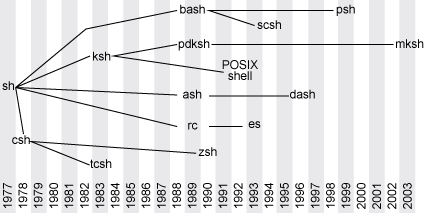
\includegraphics[width=\linewidth]{figures/misc/shells.png}}
  \caption{Linux shells since 1977, from \cite{jones2011shells} \todotext{TODO: Better quality or begone.}}
\end{figure}

\todotext{TODO: Add summaries of the features using bullet point lists.}
\todotext{TODO: Point out drawback of the features as you describe them.}
\todotext{TODO: Break up the walls of text with bold text and bullet point lists.}

\subsection{History features of C shell}

C shell (Csh) was initially released in 1978. 
It features history substitution: a simple history mechanism enabling reuse of previously executed commands inspired by Interlisp\cite{joy1994cshintroduction}. Size of the history is configurable\footnote{Examples featured in \cite{joy1994cshintroduction} and \cite{dubois1995tcshusing}
show history size set to 10 and 20 records respectively.} but according to \cite{cshman}, too large values may run the shell out of memory.

% History is disabled by default (I think) persistence accross sessions is on my install

C shell history substitution allows the user to reuse: the previous command line using \verb|!!|, the last argument of the previous command line using \verb|!$|, and all arguments of the previous command line using \verb|!*|. To run other commands lines than the previous one we could use \verb|!cc| which executes the last command line from history starting with \verb|cc|. Executing a command line based on absolute or relative index can be done using \verb|!5| or \verb|!-2| respectively. To see what command is about to be executed we could use e.g. \verb|!cc:p|, \verb|!5:p|, or \verb|!-2:p|; This only prints the history record instead of executing it. It is also possible to replace parts of command lines using \verb|!!:s/foo/bar/| or a shorthand \verb|^foo^bar| where \verb|foo| is replaced by \verb|bar| in the previous command and the result gets executed. \redtext{When using these features we do not see the resulting substituted command line until executing it. This can lead to errors or printing the substitutions first which slows users down.}
    
There is a \verb|history| command which prints out recent history records with their indexes. There are also other less notable history substitution features available; These are accessible using different modifiers that can follow \verb|!| character. Another noteworthy features of Csh are: file name tab completion, tilde expansion, command aliases, and job control.\todo{check \& ref? } \redtext{history can be easily persisted across logins}

\redtext{savehist - allows to merge history instead of overwriting it}
%savehist
%If set, the shell does 'history -S' before exiting. If the first word is set to a number, at most that many lines are saved. (The number must be less than or equal to history.) If the second word is set to 'merge', the history list is merged with the existing history file instead of replacing it (if there is one) and sorted by time stamp and the most recent events are retained. (+)
\redtext{commands lines are saved to history after the history expansion is performed}


\subsection{History features of Tenex C shell}
Tenex C shell (Tcsh) is an enhanced version of the C shell released in 1983\todo{REF}; It offers command line editing and programmable tab completion\cite{dubois1995tcshusing}. Since Tcsh is a version of C shell, it does support all the previously described features of C shell. The history holds 100 previous command lines by default and it also contains datetime of the command line execution.


Tcsh offers command line editing; This means that the user can manipulate the contents of the command line by using various built-in functions. A few examples of such functions are: \verb|delete-word|, \verb|expand-glob|, and \verb|history-search-backward|. All built-in functions can be bound to arbitrary key combinations. Additionally, Tcsh features emacs and vi editing modes which come with default keybindings usual for the respective editors. When describing the deafult keybindings for Tcsh in this section we are only considering the emacs mode.

A portion of built-in functions allows the user to reuse command lines from the shell history. Functions \verb|up-history| and \verb|down-history| allow the user to step through the history; Default keybindings are \verb|CTRL-P| and \verb|arrow_up| for \verb|up-history|; and \verb|CTRL-N| and \verb|arrow_down| for  \verb|down-history| \cite{tcshman}. This is something you are likely already used to in your modern shell.

  
% BAD ALT: Pressing \verb|CTRL-P| invokes \verb|up-history| function which replaces the current command line contents with previous command line from history. Pressing \verb|CTRL-P| repeatedly continues up through the history. Pressing \verb|CTRL-N| invokes \verb|down-history| function which steps through the history in the other direction. These two functions are also often bound to \verb|arrow_up| and \verb|arrow_down| keys. 

Besides stepping through history, Tcsh features prefix search. The functions \verb|history-search-backward| \todo{make sure this doesn't overflow :( } and \verb|history-search-forward| use the command line contents before the cursor as a prefix to search the history in the desired direction. The default keybindings for these functions are a little weird; \todo{TODO: Pressing ESC an then x is just a way of pressing ALT-x without having ALT. }
You need to press \verb|ESC| and then \verb|p| or \verb|n| for backward or forward search respectively. 

Another useful history feature of Tcsh is interactive string search. In contrast to prefix search this feature allows us to search history using any part of the command line not just the prefix. This feature is realised by \verb|i-search-back| and \verb|i-search-fwd| functions. Invoking these functions prints a secondary prompt under the primary one: \verb|bck:| or \verb|fwd:| depending on the invoked function. Typing searches the history interactively in the desired direction. Invoking the functions repeatedly steps through the history records that match the query.
These functions sound quite useful but despite that they are not bound to any keys by default.
% \redtext{So the users need to set up the key bindings themselves.}

Activating vi mode in Tcsh changes some of the keybindings. In addition to regular keybindings, stepping through history is available on keys \verb|K| and \verb|J|, and prefix search is available on \verb|SHIFT-K| and \verb|SHIFT-J|. Instead of \verb|i-search-back| and \verb|i-search-fwd| functions vi mode offers \verb|vi-search-back| and \verb|vi-search-fwd| with similar functionality.
% \redtext{vi mode has defaults - back: ? ,fwd: /}

\redtext{histdup - prunes duplicates from history}
% tcsh man page (+ means "not available in csh")
%histdup (+)
%               Controls  handling  of  duplicate  entries in the history list.  If set to `all' only unique history events are entered in the history list.  If set to `prev' and the last
%               history event is the same as the current command, then the current command is not entered in the history.  If set to `erase' and the same event is  found  in  the  history
%               list, that old event gets erased and the current one gets inserted.  Note that the `prev' and `all' options renumber history events so there are no gaps.


% Since we are mainly interested in history features we only focus on the functions that use history 
% Command line editing was an important step forward in interactive shell use. It enables the user
% As the name suggest it was inspired by features available in Tenex operating system. 

\subsection{History features of Korn shell}
Korn shell (Ksh) was initially released in 1983; It was originally written as a proprietary software until being released as open source in 2005. \todo{REF} History features of Korn shell are a very similar to the features of Tenex C shell. Ksh offers stepping through history, string search, and vi mode variant of the string search. It is worth mentioning that in Ksh, string search is bound to \verb|CTRL-R| by default which is what you are probably used to in modern shells. 

Ksh offers a shell builtin command \verb|fc| that provides a superset of C shell history mechanism\cite{rosenblatt2000kshlearning}. It allows the user to list recent history entries, edit command lines from history with an editor, and run history entries with changes. Running \verb|fc -l| lists the previous command lines from history (with indexes). So does \verb|history|, because in Ksh it is just an alias for \verb|fc -l|. To edit previous command line from history in an editor we could use \verb|fc| (without arguments) which executes the resulting command after we are done editing it. If we want to choose an editor we could use \verb|fc -e vi|. Running \verb|fc -e - foo=bar| skips the editing, replaces occurrences of \verb|foo| with \verb|bar| and executes the result. To access more then the previous command line we would use absolute or relative indexes similarly to the history expansion in Csh. For example, \verb|fc 5| and \verb|fc -2| opens an editor with fifth from the history list and the second command relative to current command line. It is also possible to select ranges of commands for editing with e.g. \verb|fc -2 -6|.

% We are not describing other Ksh history features in detail because of the similarity with already described Tcsh history features.


\subsection{History features of Bourne again shell}
Bourne again shell (Bash) was initially released in 1989.
Default history size in Bash is 500 records.\cite{bashman} Each history entry contains datetime of the execution. Unless the user disables the \verb|cmdhist| option, all lines of a multi-line command are saved as one history record; Based on \verb|lithist| option, newlines are either embeded into history or replaced by semicolons to keep the syntax of the saved commands correct. 

There are shell variables that can be used to prevent certain command lines from being saved to history. Variable \verb|HISTCONTROL| can be used to prevent saving duplicates, and to skip saving command lines starting with a space. Variable \verb|HISTIGNORE| allows using pattern matching to prevent various command lines from being saved into history.  

Bash features history expansion (\verb|!!|, \verb|!$|, \verb|!cc|, etc.) which is compatible with the Csh\cite{ramey1994gnubash}.
Bash features a \verb|histverify| option that alters the behaviour of history expansion. When it is enabled, the results of history expansion are  pasted onto the command line instead of being executed immediately. This option is disabled by default. 

\todo{COMMENTED: use this later as an example for memory load}
% It seems that authors of Bash realised the danger of history expansion; It forced the users were either forced to rely on their memory or to explicitly ask for the history expansion result to be printed first.}
% This shows us both the importance of not relying on memory/recall and the importance of adhering to the existing standard.
\todo{NOTE: we could briefly introduce Readline}
Command line editing in Bash provides most of the history related functions from Tcsh. Some of these functions have different names and some of them have different default keybindings.

Functions for stepping through history \verb|up-history| and \verb|down-history| are named \verb|previous-history| and \verb|next-history| respectively; Default keybindings did not change. 

Interactive string search (better known as reverse search) is available in Bash as \verb|reverse-search-history| and \verb|forward-search-history| with default keybindings \verb|CTRL-R| and \verb|CTRL-S|. 
Common issue with this keybinding is that \verb|CTRL-S| is often used to freeze the output of the terminal using OS's terminal driver\todo{REF: ask Barinka, he will know}; This means that many users do not have the option to search in the "forward" direction.   
Bash also provides non-interactive versions of these functions bound to \verb|ALT-P| and \verb|ALT-N|. However, besides saving your CPU from searching the history multiple time, they do not seem to provide any advantage over their interactive counterparts. 

Prefix search functions are still available under the same name (\verb|history-search-backward| \todo{overflow!} and \verb|history-search-forward|) but they do not have default keybindings in Bash. Alternative substring searching versions for these functions are available which do not search just by prefix but can match anywhere on the command line: \verb|history-substring-search-backward| and \verb|history-substring-search-forward|.\todo{overflow!}

Another two history functions we can find in Bash are \verb|yank-last-arg| and \verb|yank-nth-arg|. The first one pastes the last argument of the previous history entry onto the command line. The second one pastes the Nth argument. Default keybindings for \verb|yank-last-arg| are \verb|ALT-.| or \verb|ALT-_|. To use \verb|yank-nth-arg| we need to provide an argument to Bash input library; This can be done by pressing an \verb|ALT| key with a numeric argument. Then we can press \verb|CTRL-ALT-Y|. Without providing any argument the function pastes the first argument of the previous history entry onto the command line.


Other than command line editing functions Bash offers builtin commands to list, reuse and manipulate the history. The \verb|fc| builtin is very similar to the one available in Ksh. We can list of recent command lines from history with \verb|fc -l|, edit and execute them with \verb|fc| without any arguments, and substitute and execute them with \verb|fc -s foo=bar|. It is possible to select command lines and ranges of command lines from the history using absolute or relative indexes.

Compared to Ksh, \verb|history| is no longer just an alias; It is a Bash builtin which can be used to display and control the shell history. Without any arguments, \verb|history| prints out a list of previous history entries with indexes. Using various command line options it can be used to: add command lines to history, delete them, or clear the history. It can load new or all history entries from the history file to the history of this shell session; New entries could appear in the history file because of other simultaneously running shell sessions. Conversely, we can use the \verb|history| builtin to append or write the history of this shell session to the history file.


\subsection{History features of Z shell}

Z shell (Zsh) was originally released in 1990. Most of the history features available in Bash are also offered by Zsh.
The default history size is just 30 lines. The history contains the executed command line, the datetime and the duration of the execution. This information is only saved to history when the \verb|EXTENDED_HISTORY| option is enabled. 

% Zsh is overall more feature-rich than Bash. 
% Many features and options that are natively supported in Zsh are non-trivial or impossible to set up in Bash\todo{example?, ref?}.
% We are not going to cover Zsh in great detail because of its similarity to Bash.

Zsh does feature csh-style history expansion. Like Bash, it can be configured to evaluate the history expansion and paste the result onto the command line instead of executing it; This behavior can be enabled using \verb|HIST_VERIFY| option. Another way to see what the history expansion evaluates to is the \verb|magic-space| function. It evaluates history expansion and inserts a space when invoked. When we bind this function to spacebar the history expansion will get evaluated every time we press \verb|SPACE|.

\todo{NOTE: we could briefly introduce ZSH ZLE}
We can find Zsh equivalents for almost all Bash command line editing functions that allow history reuse. In addition, we can find variations and extra functions compared to what is available in Bash. Using \verb|arrow_up| and \verb|arrow_down| keys we can retrieve recent command lines from history. Prefix search is available but unbound by default. There is a variant of prefix search that always searches by first word on the current command line no matter where the cursor is. This variant of prefix search is bound to \verb|ALT-P| and \verb|ALT-N| by default. Interactive reverse search functions are also available with the same default keybindings as in Bash.

Zsh offers pattern matching variants for the most of the history searching functions; These treat the typed query as a pattern instead of a string that should be matched exactly. Vi mode variants for some of the searching functions are available as well.  

The \verb|fc| builtin command is supported and the functionality is comparable to its Bash counterpart. Like in Ksh, \verb|history| is just an alias for \verb|fc -l|. 

% There are alternatives to achieve almost anything that can be done in Bash. For example, ...


\blind
\todotext{TODO: short conclusion about shells ? }


\section{How people use shell and shell history}

In this chapter we examine how people use shell and shell history.

1) Consider previous research that studies the properties of how people use command based systems

2) 

To do so we consider previous research on the topic which features an analysis of ... 


\todotext{TODO: how do standard shell history features relate to the way people use shell}

\todotext{TODO: intro - why we need to study the ways people use shell and shell history }

\blind[2]



\subsection{Collecting shell history}



\subsection{How people use shell - split into more subsections?}



\todotext{Frequency distributions of commands}

\redtext{ Zipf distribution, which has the property that a relatively small number of items have high usage frequencies, and a very large number of items have low usage frequencies}

\redtext{ A looser characteristic of this kind of rank distribution is the well-known 80-20 rule of thumb that has been commonly observed in commercial transaction systems - 20\% of the items in question are used 80\% of the time (Knuth, 1973; Peachey,Bunt, and Colbourn, 1982).2}
 \redtext{In measurements recorded from a UNIX site, Hanson, Kraut, and Farber (1984) report a similar trend - 10\% of the 400-500 commands available account for 90\% of the usage}

\redtext{ME: We have collected contextual shell history from a number of people }

\todotext{TODO: describe how the plot was created}

\redtext{ME: Our newly collected data matches the distribution found in greenberg study}

\redtext{ME: Based on our data ... }

\redtext{Top 10 \% of cmds amounts for 65.5061446260756 \% of all command lines}
\redtext{Top 20 \% of cmds amounts for 79.95709255415899 \% of all command lines}
\redtext{ME: Our data follow the 80-20 rule but it's still a difference compared to the stats from the study - we suspect that difference is mainly caused by larger number of commands used by the users overall}



\redtext{Top used commands differ between people - }
\redtext{According to greenberg, even when people have very similar expertise and identical goals the commands they use vary significantly. - Our data is in line with this idea.} 


\todotext{Vocabulary}

\redtext{Command vocabulary is the set of commands used by a given person. We are interested in analysing how the vocabulary of the user changes over time.}

\redtext{Greenberg reports adoption or about 5\% for all users before they enter 1k command line. They conclude that this is an initial learning period when the system encounters most of the commands for the first time. According to Greenber, after initial 1k cmd lines entered the adoption rate drops quicky under 1\%. This is somewhat in line with our findings. We did observe about 5\% cmd adoption rate during the first 1k cmdlines entered for vast majority of our users. Between 1k and 2k we saw a drop in adoption of new commands to about 3\%. Between 2k and 3k the adoption dropped to numbers between 1\% and 2\% for most users. Most users would eventually drop to a stable adoption rate of anywhere between 1 to 3\%.}

\redtext{This difference could be caused by multiple factors. There is more commands available compared to XX years before. Additionally, custom commands/scripts seem to be very common in our data while they seem to be non-existent in the greenberg study. This alone could have a huge impact. Draper (see below) was referring to a number of commands available to users of ... as 570. }

\redtext{Nowadays the number of available commands is virtually unlimited because users can install and create new commands. Number of initially available commands on a newly installed system is in thousands.}

\redtext{ REF: Draper (1984) estimated the times a command was invoked by noting the UNIX processes spawned during each user's interaction with the system (method 4, Section 2.2.1).5 He suggested that the overall trends observed are representative of real command use. First, out of a vocabulary of the 570 commands available to the population, only 394 (70\%) were used at least once. }

\redtext{We can conclude that command usage distribution was and still is very uneven (few commands dominate the distribution) and that the number of available commands significantly increases over time.}

% eva: Cmd adoption rate at 1k cmdlines = 0.054
% eva: Cmd adoption rate at 2k cmdlines = 0.044
% eva: Cmd adoption rate between 1k and 2k cmdlines = 0.034
% eva: Cmd adoption rate between 2k and 3k cmdlines = 0.01
% eva: New cmd adoption rate after 1k cmdlines = 0.012322801815991847
% eva: New cmd adoption rate after 2k cmdlines = 0.010109261717553355
% simon: Cmd adoption rate at 1k cmdlines = 0.087
% simon: Cmd adoption rate at 2k cmdlines = 0.061
% simon: Cmd adoption rate between 1k and 2k cmdlines = 0.035
% simon: Cmd adoption rate between 2k and 3k cmdlines = 0.016
% simon: New cmd adoption rate after 1k cmdlines = 0.022236340533672173
% simon: New cmd adoption rate after 2k cmdlines = 0.018807092960773777
% tivvit: Cmd adoption rate at 1k cmdlines = 0.054
% tivvit: Cmd adoption rate at 2k cmdlines = 0.0375
% tivvit: Cmd adoption rate between 1k and 2k cmdlines = 0.021
% tivvit: Cmd adoption rate between 2k and 3k cmdlines = 0.022
% tivvit: New cmd adoption rate after 1k cmdlines = 0.014787430683918669
% tivvit: New cmd adoption rate after 2k cmdlines = 0.01411790063584438

\redtext{??? When collecting history there is always an initial period where we encounter many new commands at a high rate because the current vocabulary is very small. This part is expected as we notice commands for the first time Part of the curve after the initial "steep" period represents the rate of adopting new commands by users. Some new commands are adopted because of new tasks and goals of the user. Some commands seem ... }



\todotext{Sequences}

\redtext{toolsmith and the original sequence graph talked about how individuals have }




\todotext{TODO: Greenberg conducted a study in his work \cite{greenberg1993computer} in 19XX which provides a lot of insight into how people use shell. It's not obvious that conclusions and ideas in the work still hold. To make sure that the usage of shell didn't change to the point where we can't use the ideas anymore. }

\todotext{TODO: Predicting users' next command line - what is the state of the art, what are the disadvantages}

\todotext{TODO: Sequential relationships of commands}

\blind[4]
% plots:

% Figure 3.1. The normalized command frequency, compared with Zipf.

\begin{figure}
  \tmpframe{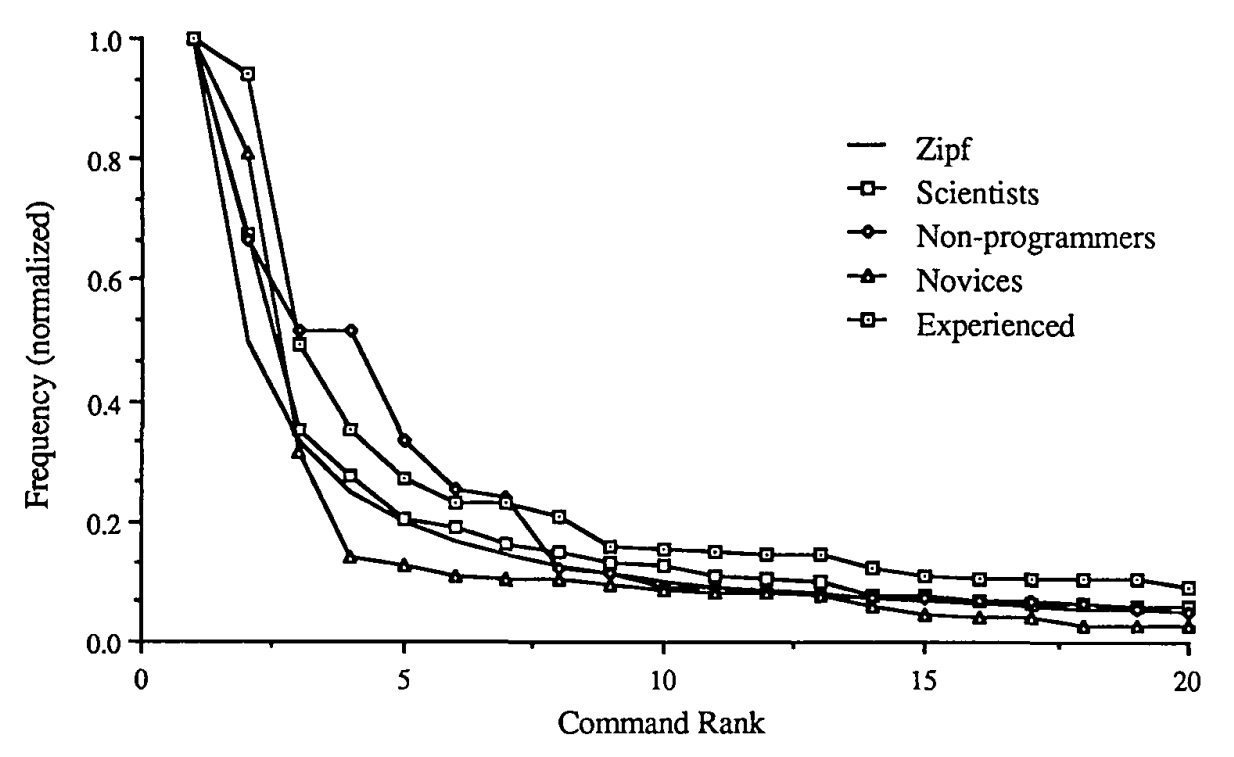
\includegraphics[width=\linewidth]{figures/greenberg/plot_ref_zipf-cmd-frq.png}}
  \caption{The normalized command frequency, compared with Zipf. (Greenberg)}
\end{figure}

\begin{figure}
  \tmpframe{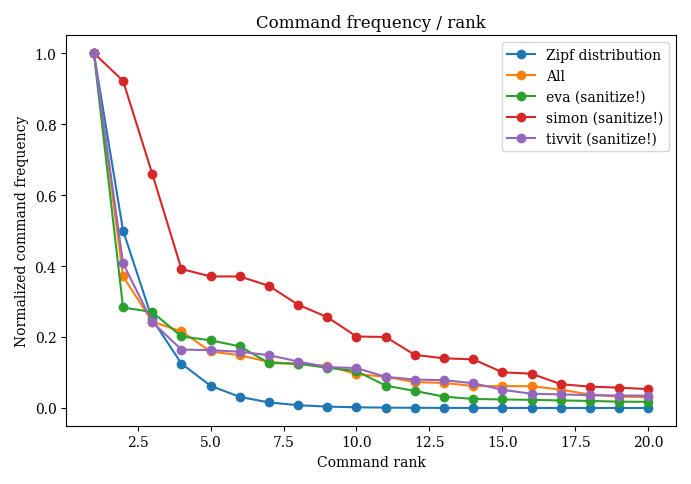
\includegraphics[width=\linewidth]{figures/greenberg_new/plot_zipf-cmd-frq.png}}
  \caption{The normalized command frequency, compared with Zipf. \todotext{unify labels to match Greenberg, export in vector, lose top title, add data from more people, have one line for each person and then one line for all people together}}
\end{figure}
\todo{make sure figures are not all over the place}

% Figure 3.2. Command vocabulary size vs. the number of command lines entered for four individuals.

\begin{figure}
  \tmpframe{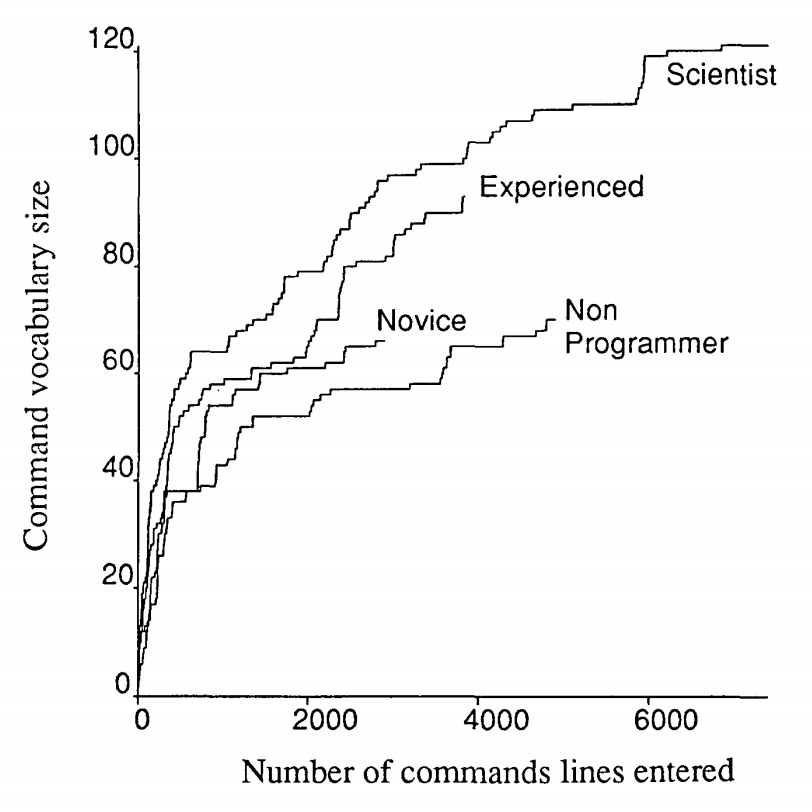
\includegraphics[width=\linewidth]{figures/greenberg/plot_ref_cmd-vocab-size.png}}
  \caption{Command vocabulary size vs. the number of command
lines entered for four individuals. (Greenberg)}
\end{figure}

\begin{figure}
  \tmpframe{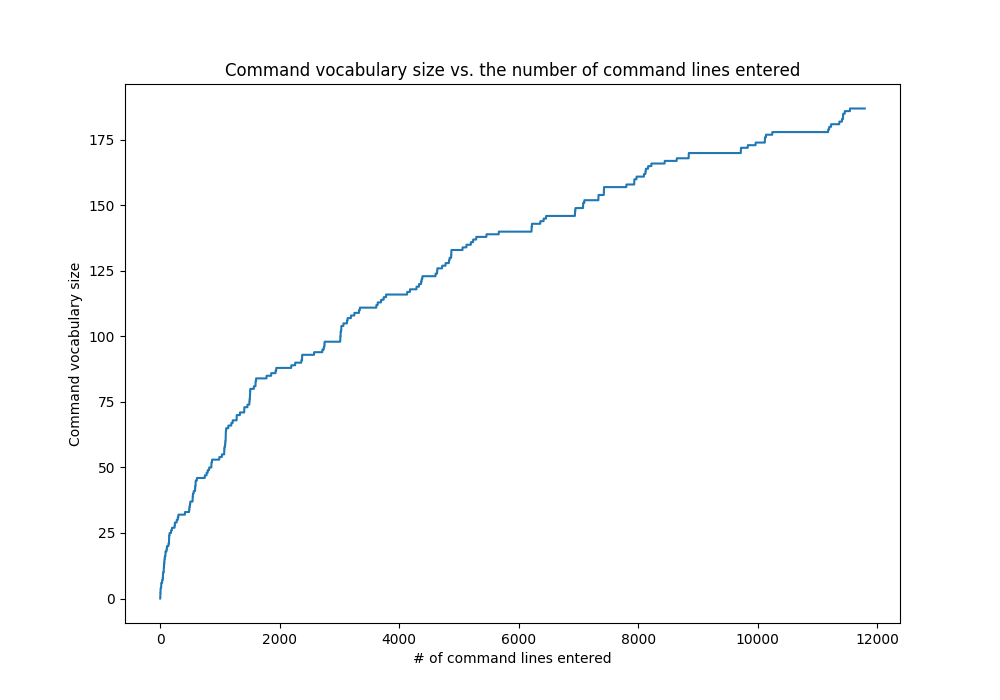
\includegraphics[width=\linewidth]{figures/greenberg_new/plot_cmd-vocab-size.png}}
  \caption{Command vocabulary size vs. the number of command
lines entered for \todotext{N individuals}}
\end{figure}


% Figure 3.3. Sequential structure of UNIX command usage, from Figure 4 in Hanson et al. (1984).

\begin{figure}
  \tmpframe{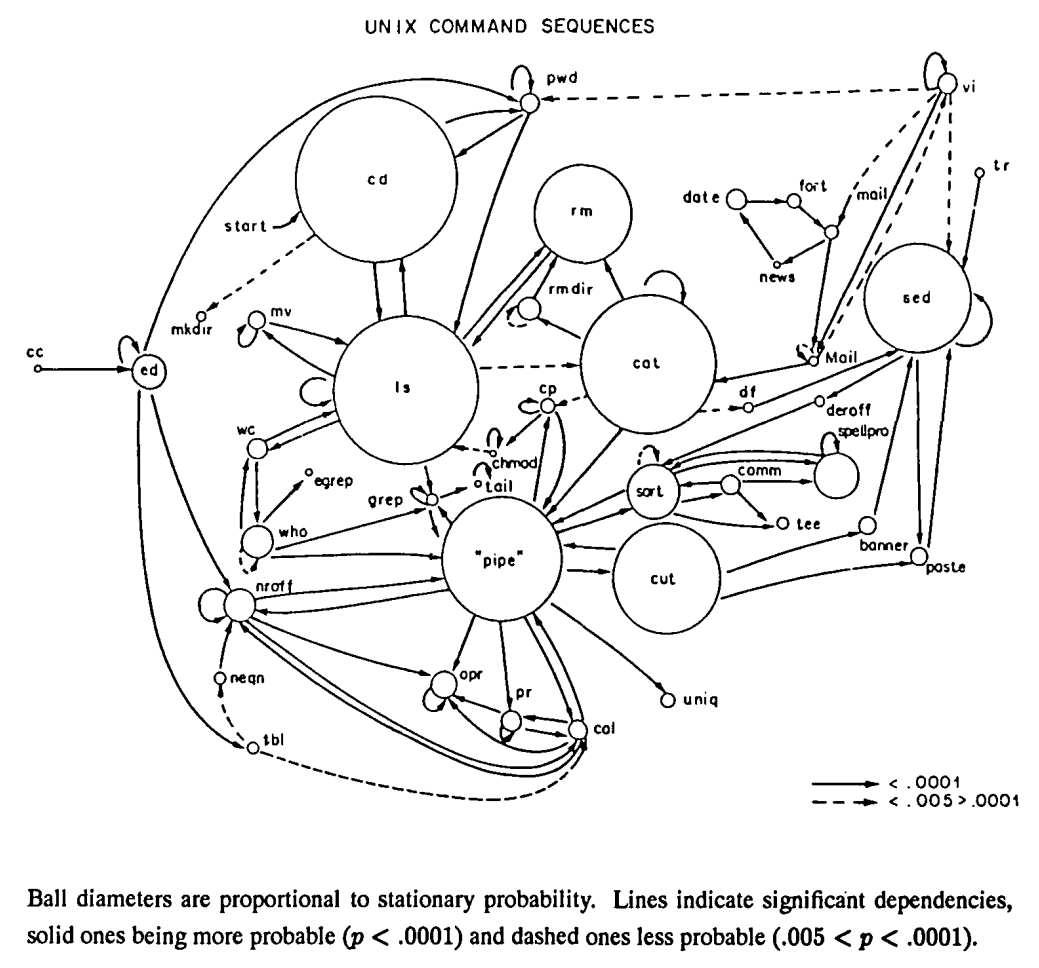
\includegraphics[width=\linewidth]{figures/greenberg/graph_ref_cmd-sequences.png}}
  \caption{Sequential structure of UNIX command usage, from Figure 4
in Hanson et al. (1984). (Greenberg)}
\end{figure}

\begin{figure}
  \tmpframe{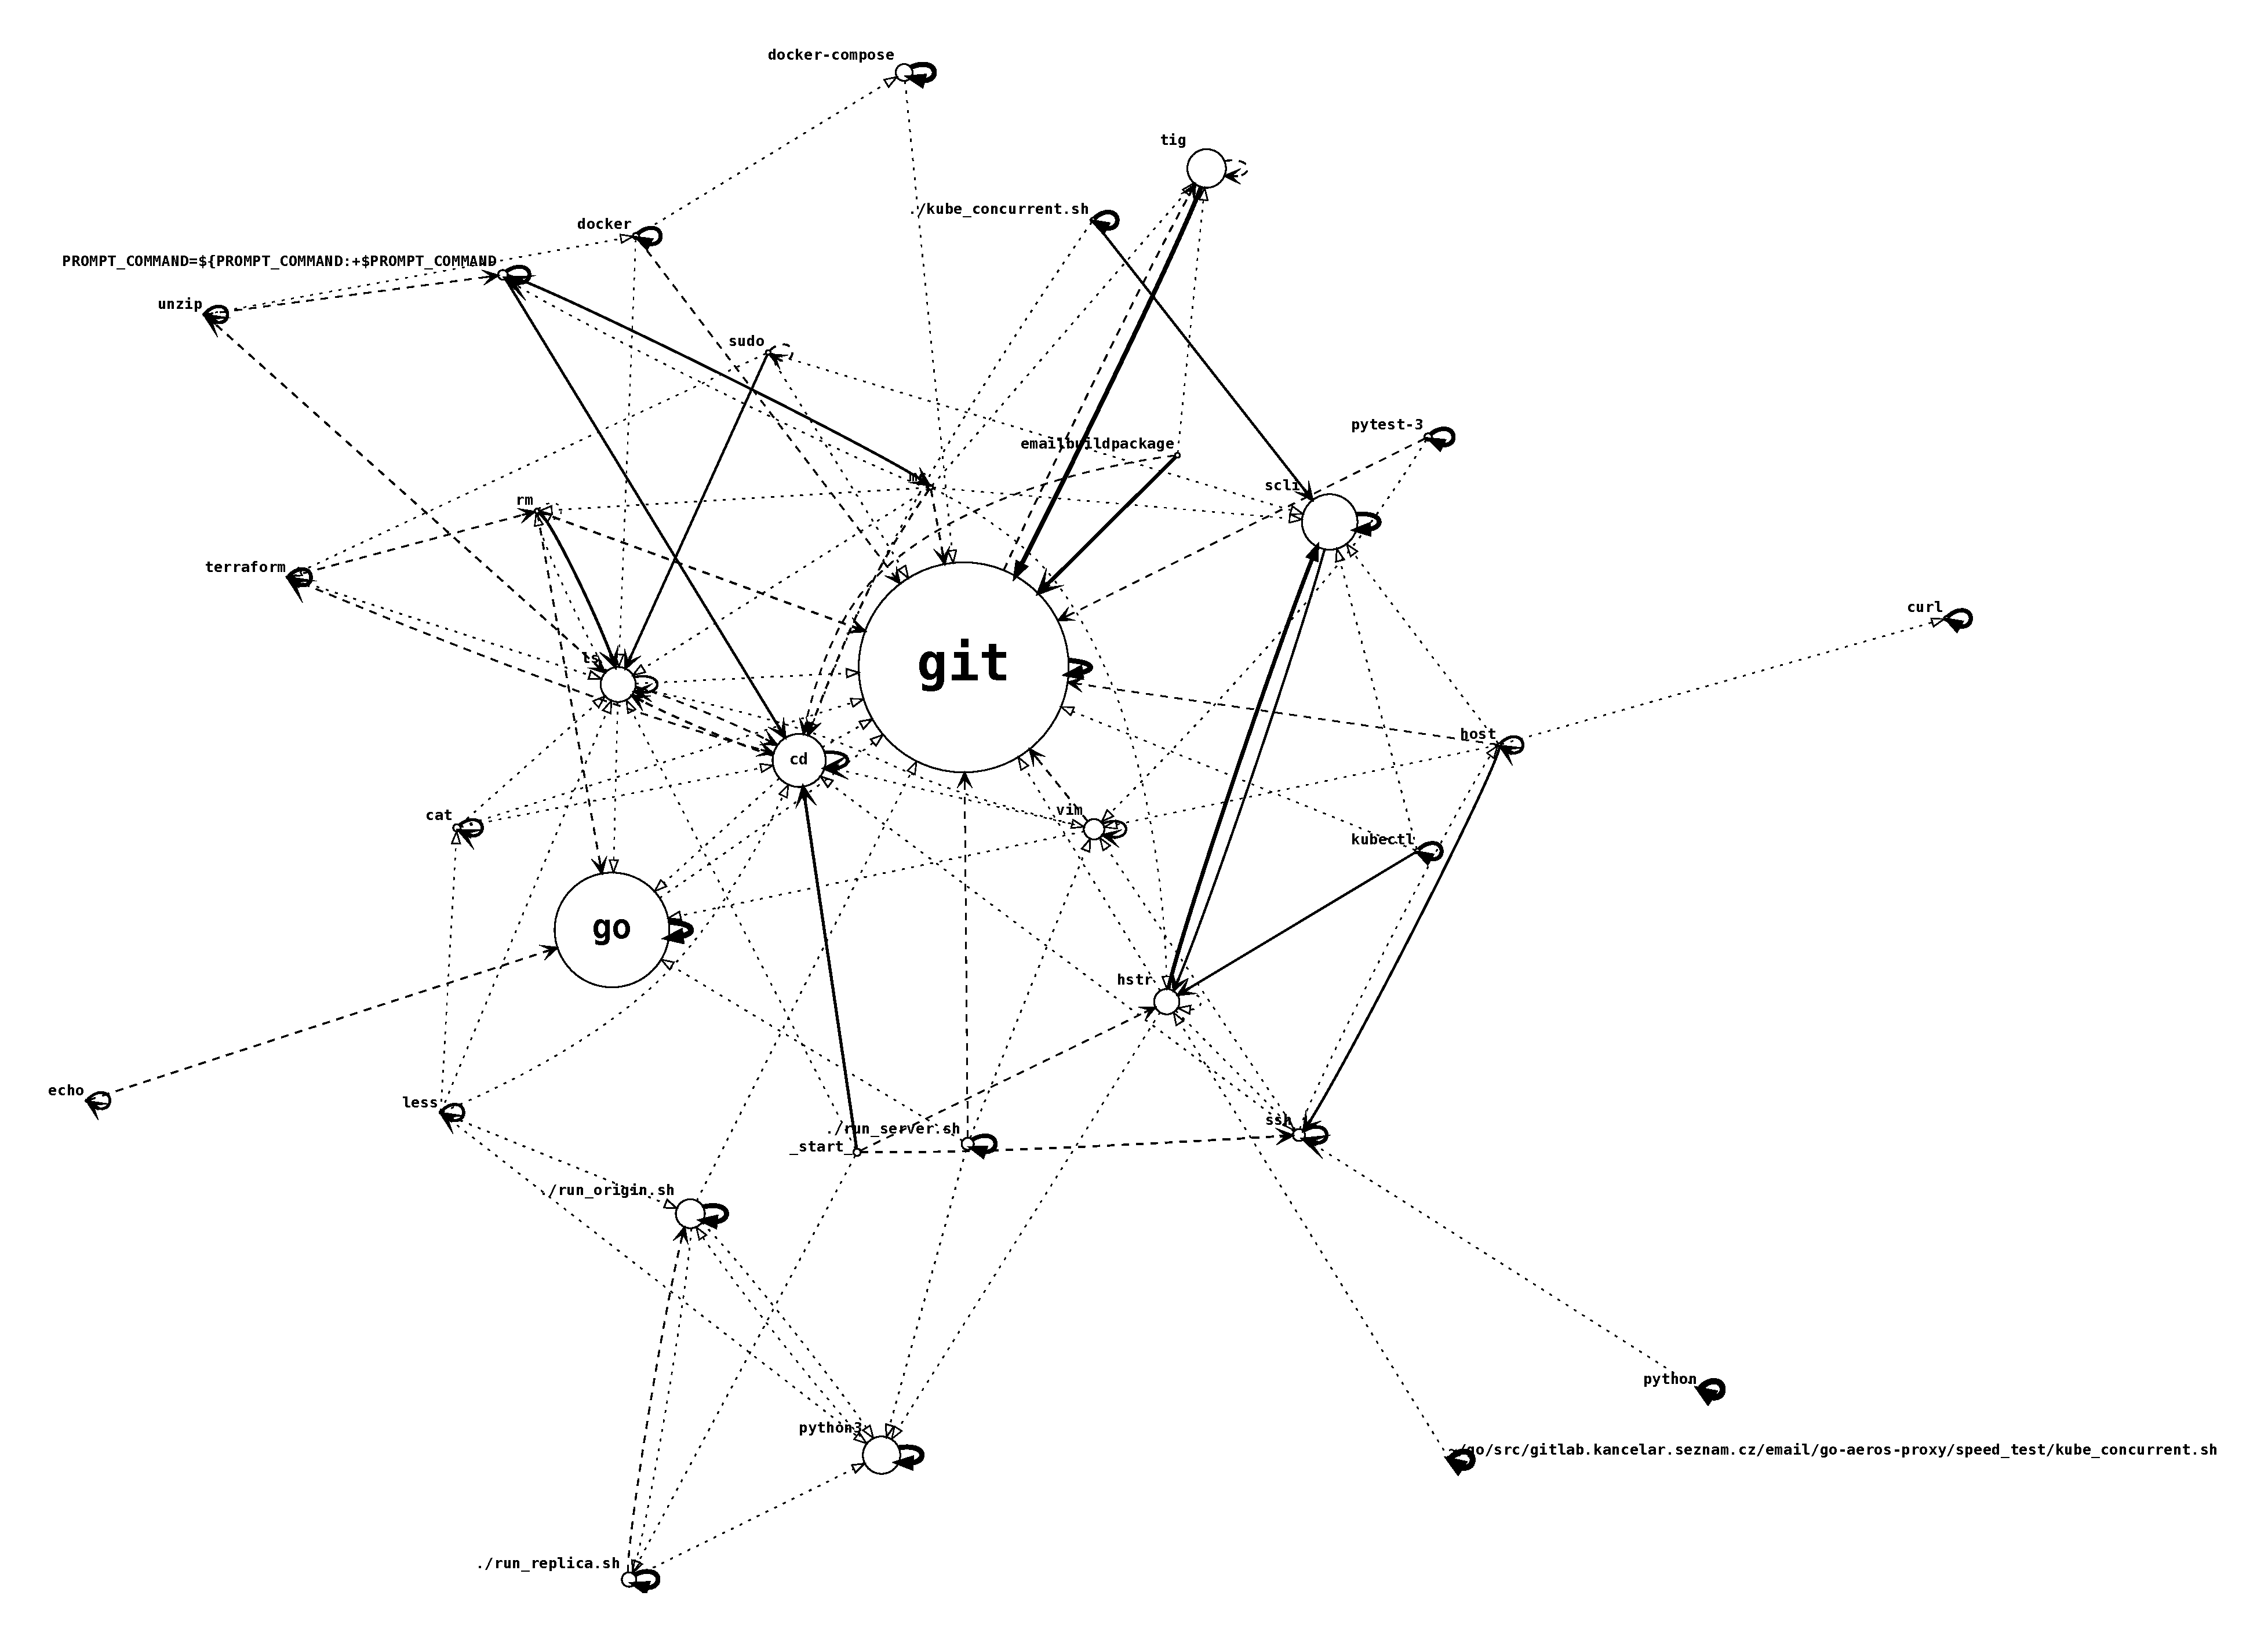
\includegraphics[width=\linewidth]{figures/greenberg_new/graph_cmd-sequences.pdf}}
  \caption{Sequential structure of command usage. \todotext{Make this more narrow so the text is bigger}}
\end{figure}


% Table 5.2. The average recurrence rate of the four sample UNIX user groups

\begin{figure}
  \tmpframe{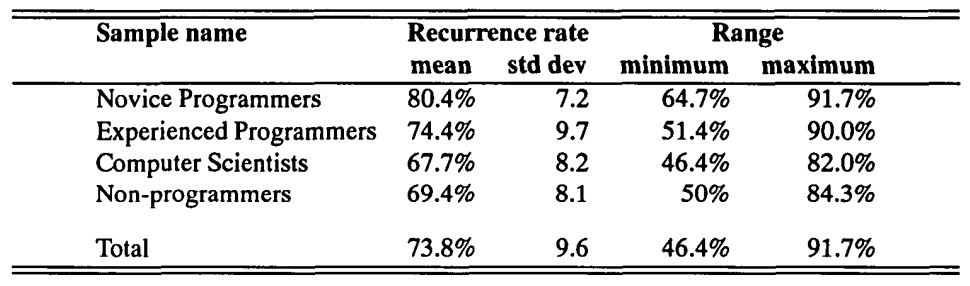
\includegraphics[width=\linewidth]{figures/greenberg/table_recurr-rate-in-different-samples.png}}
  \caption{The average recurrence rate of the four sample UNIX user groups (Greenberg) \todotext{redo as an actual table}} 
\end{figure}

% Figure 5.6. Command line vocabulary size vs. the number of commands entered for four typical individuals.

\begin{figure}
  \tmpframe{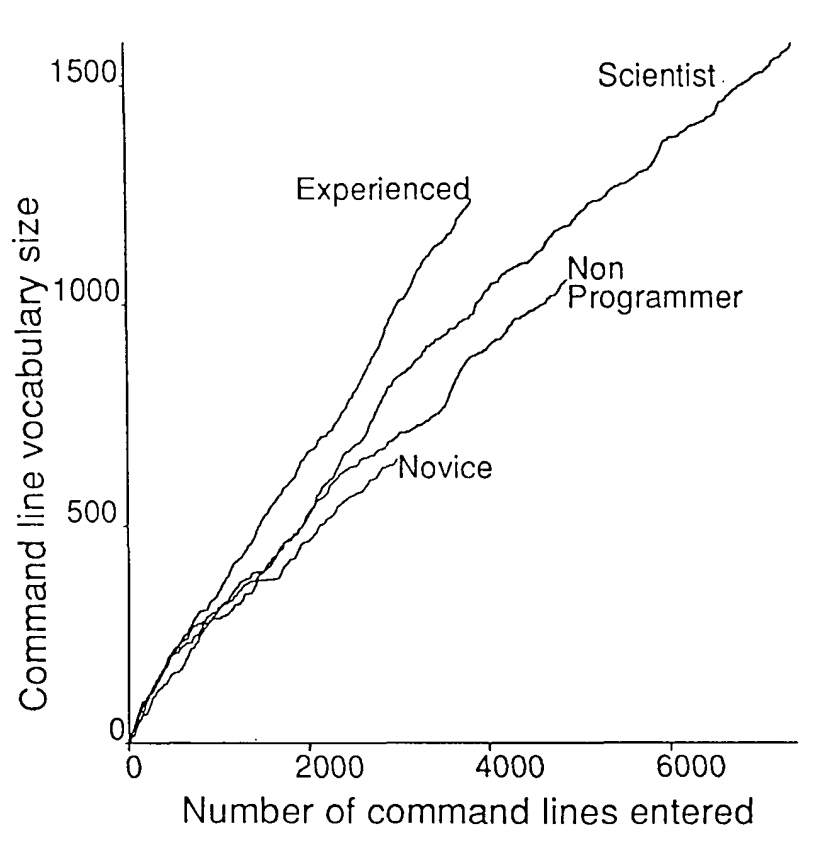
\includegraphics[width=\linewidth]{figures/greenberg/plot_ref_cmdline-vocab-size.png}}
  \caption{Command line vocabulary size vs. the number of commands
entered for four typical individuals. (Greenberg)}
\end{figure}

\begin{figure}
  \tmpframe{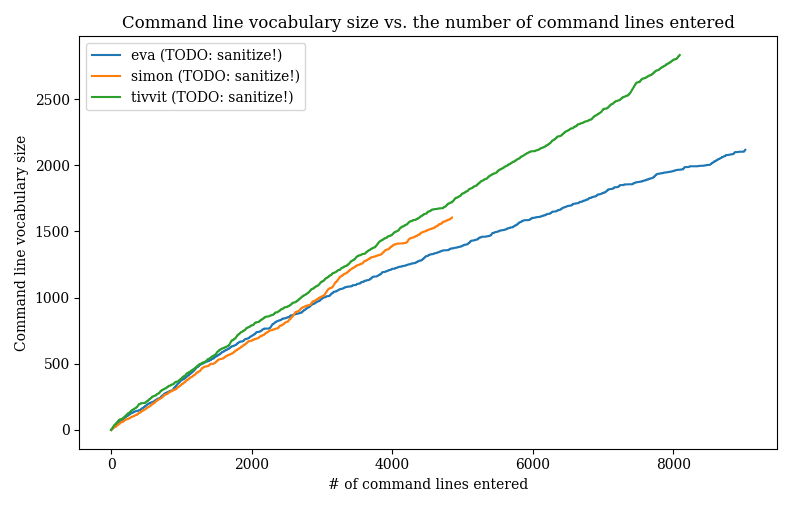
\includegraphics[width=\linewidth]{figures/greenberg_new/plot_cmdline-vocab-size.png}}
  \caption{Command line vocabulary size vs. the number of commands
entered for a single experienced programmer \todotext{TODO: title}}
\end{figure}

% greenberg 1993 vs now
% the average length of command lines is 7.58
% recurrence rate is 74.4% for Experienced Programmers (avg group), max chars. recalled for an optimal conditioning method is 4.43 characters predicted per submission.


\todotext{How have shell usage changed since standard shell history features and greenberg study - longer commands, more commands; sessions (there can be more terminal windows open -> history is not strictly sequential anymore); }

\todo{avg recurrence rate \& avg max possible recalled characters}
% together (beware there is a lot of me - cleanup and redo)
%>>> Top 10 %% of cmds amounts for 65.5061446260756 %% of all command lines
%>>> Top 20 %% of cmds amounts for 79.95709255415899 %% of all command lines
%>>> Avg recurrence rate = 70.28292049957133
%>>> Max avg recalled characters = 17.345876682809276
%>>> Max avg recalled characters (including prefix matches) = 26.93303519707116

%tivvit
%>>> Top 10 %% of cmds amounts for 58.38949982263214 %% of all command lines
%>>> Top 20 %% of cmds amounts for 73.26179496275275 %% of all command lines
%>>> Avg recurrence rate = 65.21241973788372
%>>> Max avg recalled characters = 17.545342598293605
%>>> Max avg recalled characters (including prefix matches) = 30.283226317178293
%w/o errors
%>>> Avg recurrence rate = 65.3752138841359
%>>> Max avg recalled characters = 16.457467611830847
%>>> Max avg recalled characters (including prefix matches) = 28.687973600586652
%eva
%>>> Top 10 %% of cmds amounts for 60.87177747625509 %% of all command lines
%>>> Top 20 %% of cmds amounts for 79.68113975576662 %% of all command lines
%>>> Avg recurrence rate = 77.79189967802067
%>>> Max avg recalled characters = 15.405016098966277
%>>> Max avg recalled characters (including prefix matches) = 22.08049483138451
%w/o errors
%>>> Avg recurrence rate = 76.5637108380383
%>>> Max avg recalled characters = 15.118897376286949
%>>> Max avg recalled characters (including prefix matches) = 22.381932912653603
%me @ seznam
%>>> Top 10 %% of cmds amounts for 57.32517482517483 %% of all command lines
%>>> Top 20 %% of cmds amounts for 68.0944055944056 %% of all command lines
%>>> Avg recurrence rate = 65.33170816646351
%>>> Max avg recalled characters = 18.805850600731326
%>>> Max avg recalled characters (including prefix matches) = 33.09333101166638
%w/o errors
%>>> Avg recurrence rate = 66.93366194290408
%>>> Max avg recalled characters = 18.43787225302937
%>>> Max avg recalled characters (including prefix matches) = 31.69172314643664


\blind[4]


\subsection{How people use shell history}
\todo{practical chapter with concrete examples based on the standard history features}

\todotext{TODO: intro}

\blind 

\todotext{TODO: talk about our online research - my twitter thread, hackernews threads, SO questions, etc.}
\todotext{TODO: features people want, ask for; opinions, ...}

\blind

\todotext{TODO: introduce personas - HERE?!}
\todotext{TODO: describe use cases - HERE?! - yes because we want to compare the standard history features to our solution in the end using these use cases }

\todotext{USECASE: use case where we find something in history and want to find a similar command immediately: 1 use resh cli to find the first command, 2 execute, 3 arrow\_up, 4 ctrlR gives you similar results to what you found before}

\todotext{USECASE: come back to a project and continue previous work on it}

\todotext{USECASE: fix a typo in a previous command}

\todotext{USECASE: use: sudo !! to run a previous command with sudo}

\todotext{USECASE: find a long (w/ many arguments/options) curl request to github api}

\todotext{USECASE: run a recent git command}

\todotext{USECASE: find a command using datetime, command(first word) }

\blind[4]

\todotext{TODO: conclusion of the chapter}

\blind

\section{Existing history tools and common history configurations}
\todo{chapter with various possible solutions, inspirations, etc.}

\todotext{TODO: mention our online research again}
\todotext{TODO: shell history configurations options}



\subsection{Existing history tools \todotext{TODO: split into more subsections}}

\todotext{TODO: common configuration options and what problems are they solving}

\todotext{TODO: configuration management projects e.g.: oh-my-zsh}

\todotext{TODO: }

\subsection{History features of Read-eval-print loops}

\subsection{History features of Friendly interactive shell}

\todo{more subsections ...}
\blind[1]

\blind[4]

\todotext{TODO: short conclusion about history tools, configurations, etc.}



\section{Available contextual information}

\todotext{TODO: intro}

\subsection{Directly available contextual information}

\blind[2]

\subsection{Derivable contextual information}

\blind[2]

\subsection{Usage of history features as a context}

\blind[2]

\todotext{TODO: conclusion of the section}



\chapter{Design}
\todotext{TODO: intro describe contents of the chapter}

\blind
\todo{order of design chapters can change}
\section{Recording contextual history}

\todotext{TODO: what to record}

\blind[2]

\section{Interactive history features} % front-end

\todotext{TODO: intro}

\blind

\subsection{Standard history features}

\todotext{TODO: describe why it's important to respect the standard history features}

\todotext{TODO: which history features are we keeping/enhancing/leaving intact}

\blind[3]

\todotext{TODO: conclusion for further design ?}



\subsection{Core ideas, principals, design decisions, and features}\todo{weird title}

\todotext{TODO: intro: ideas in this chapter are essential for this work / project}

\todotext{TODO: features of the project - weird todo}

\blind[3]

\subsection{Possible features}

\todotext{TODO: intro: this section describes features that were considered during the design - for each feature we evaluate how well it would fit with the rest of the design. Some of the features were explicitly suggested by users and some features are included for the sake of completeness (because they make sense).}

\todo{TODO: list the features}


\section{Back-end}\todo{I don't like the title}

\blind

\section{Testing the design}

\todotext{TODO: explain why we want to test the design - intro}

\todotext{TODO: principals, guidelines, etc. are we are using}

\blind[3]

\chapter{Implementation}
\todo{merge sections to have less of them}
\todotext{describe layout/contents of the chapter}

\blind

\section{Daemon}\todo{do we need this or is introduction enough}

\blind

\section{Choosing Go}

\blind[3]

\section{Recording shell history with context}

\blind

\subsection{History format}

\todotext{NOTE: both on disk and in transfer}

\blind

\subsection{Shell integration and hooks}

\blind

\subsection{History record merging}

\blind

\section{Custom arrow key bindings}

\todotext{TODO: intro: we want arrow key bindings to be able to record usage related metadata + it's a good idea to have the option to customize and use context to enhance arrow key bindings. Plus impossibility of gathering usage data and using the default bindings (at least in Bash)}

\blind

\subsection{Keybinding custom functions in zsh}

\blind

\subsection{Keybinding custom functions in Bash}

\blind

\subsection{Reverting keybindings}

\blind

\subsection{Universal keybinding library}
\todotext{TODO: explain why: as you see Bash and zsh have a different ways of supporting custom keybindings. To simplify our codebase we extracted the keybind setting logic into a library. (unified way to set keybindings)}

\blind

\subsection{Performance issues of custom keybindings in Bash}

\blind


\section{Fullscreen command line history searching application}

\todo{TODO: subsections}


\section{Daemon components}

\todotext{TODO: describe why we need components}

\begin{figure}
  \tmpframe{\includegraphics[width=\linewidth]{figures/daemon-components.jpg}}
  \caption{One image. \todotext{TODO: write a title}}
  \label{fig:TODO}
\end{figure}

\subsection{Server}

\subsection{History file}

\subsection{Session history}
\todotext{TODO: explain: there are implications for the daemon if we want responsive arrow key bindings}

\subsection{Expired session tracking}


\subsection{Signal handling}

\blind

\section{Control and configuration}

\blind

\section{Installation, updates, and build process}

\todotext{TODO: explain how simple the installation is. plus updates.}

\blind

\subsection{Installation and updates}
\todotext{TODO: explain how installation works}

\blind

\subsection{Production and development build process}
\todotext{TODO: explain the build process}

\blind[2]


\chapter{Testing and Evaluation}

\todotext{TODO: describe layout/contents of the chapter}

\todotext{TODO: describe how history tools can be usable}

\todotext{TODO: describe what influences usability of the tools}

\todotext{TODO: explain which parts of the system should be tested and why}

\blind[3]

\section{Metrics}

\todotext{TODO: describe why we use metrics}

\subsection{Metrics traditionally used to evaluate history tools}\todo{break down into more subsections ?}

\todotext{TODO: describe which metrics were used for history tools in the past}

\subsection{Newly suggested metrics}\todo{break down into more subsections ?}

\todotext{TODO: suggest new metrics + explain how they are better than the original ones}

\subsection{Evaluation using suggested metrics}

\todotext{TODO: explain used methods}

\todotext{TODO: use metrics to evaluate usefulness of the work}


\section{Use cases}



\begin{conclusion}

\todotext{TODO: rewrite conclusion}

I have analysed shell history features available in current shells. I explored available history tools and found both positive and negative inspiration.

\par I have found previous research on how people use shell and shell history.  
I have collected a sample of shell history. I have analyzed the collected usage data and compared it to data used in existing research. I have found which characteristics of shell usage changed over time and which characteristics stayed the same. I have concluded that most of the principals and ideas from the existing research do still hold. I have found out that potential recalled characters increased 4 times since the study was conducted. This and other differences reinforced the idea that it makes sense to design and develop new history related tools. 

\par I have conducted a market research to find out how people interact with shell history and what are the workflows that are not well supported nowadays. I have modelled personas representing target users of the system. I have put together use cases based on actual shell history I have collected.
I have designed a contextual shell history tools based on problems and suggestions from existing literature, user-centered design guidelines and principals, information learned via market research, and modelled personas.
I have actively sought feedback from users during both design and implementation. 

I have used usability principals and heuristics to test and evaluate the design.

\par I have implemented a significant portion of the design. The project unobtrusively records shell history with context. It does both use context to offer relevant history records and for searching via fullscreen command line application.
I have made sure that it's easy to install, update, configure and use. I have shared the resulting implementation with community and received overwhelmingly positive feedback and interest of contributors. Project was downloaded and installed over 5 hundred times since January. Github page of the project consistently attracts daily visitors.  

\par I have described a number of possible metrics. I have explained why simple metrics are not sufficient. I have described the drawbacks of metrics in general. I have suggested meaningful metrics that can be used to evaluate shell history tools. I have used the suggested metrics to evaluate my implementation where possible. 

\par I have used modelled personas and use cases to evaluate utility and usability of the system.
I have used real life user data to evaluate user experience of the solution.


I have made it easier to collect and study usage of shell and shell history in future research.
I have proved that having contextual shell history brings many benefits. 
I have demonstrated public demand for history tools. 
I have created a universal shell library for binding custom functions to keys with the option to revert to previous state. 




\todotext{TODO: write future work}

\end{conclusion}

\bibliographystyle{iso690.bst}
\bibliography{ref}

\appendix

%\printglossaries

\chapter{Contents of SD card}\label{app:SDcontent}

\todotext{TODO: Visualise the contents of enclosed media. Use of dirtree is recommended. Note that directories src and text with appropriate contents are mandatory.}


\begin{figure}
	\dirtree{%
		.1 readme.txt\DTcomment{the file with CD contents description}.
		.1 data\DTcomment{the data files directory}.
		.2 graphs\DTcomment{the directory of graphs of experiments}.
		.3 *.eps\DTcomment{the B/W graphs}.
		.3 *.png\DTcomment{the color graphs}.
		.3 *.dat\DTcomment{the graphs data files}.
		.1 exe\DTcomment{the directory with executable WBDCM program}.
		.2 wbdcm\DTcomment{the WBDCM program executable (UNIX)}.
		.2 wbdcm.exe\DTcomment{the WBDCM program executable (Windows)}.
		.1 src\DTcomment{the directory of source codes}.
		.2 wbdcm\DTcomment{the directory of WBDCM program}.
		.3 Makefile\DTcomment{the makefile of WBDCM program (UNIX)}.
		.2 thesis\DTcomment{the directory of \LaTeX{} source codes of the thesis}.
		.3 figures\DTcomment{the thesis figures directory}.
		.3 *.tex\DTcomment{the \LaTeX{} source code files of the thesis}.
		.1 text\DTcomment{the thesis text directory}.
		.2 thesis.pdf\DTcomment{the Diploma thesis in PDF format}.
		.2 thesis.ps\DTcomment{the Diploma thesis in PS format}.
	}
\end{figure}


\end{document}
